\documentclass[11pt,twoside,a4paper]{report}
\usepackage{appendix}
\usepackage{geometry}
\usepackage{graphicx}
\usepackage{pdfpages}

% set the default, standard, geometry
\geometry{left=25mm, right=25mm, top=25mm, bottom=25mm}

\setlength{\parskip}{\baselineskip}
\clubpenalty10000
\hyphenpenalty10000
\widowpenalty10000

\begin{document}

\title{ID2216 Developing Mobile Applications\\Assignment 3 Report}
\author{Rafael Aldana (rafaelap@kth.se)\\Vincent Delitz (delitz@kth.se)\\Ruth Eriksson (ruthe@kth.se)}
\date{\today}
\maketitle

%\newcommand{\webOrNative}{Web~}

%\begin{abstract}
%During the course, we have worked in team to propose, build, and document a mobile app. We have developed a functional \webOrNative application that addresses an interesting and relevant area we have identified. This report describes step-by-step how we designed the mobile application.
%\end{abstract}

\tableofcontents
\thispagestyle{empty}

%\listoffigures

%\listoftables

\renewcommand{\chaptername}{Assignment}
\setcounter{chapter}{1}
\chapter{WebApp Prototype}
\setcounter{page}{1}

\section{WebApp prototype feedback}

After finalizing the WebApp prototype, we showed it to friends in order to gather their feedback. Some of the major feedback points we discovered are listed below:

\begin{itemize}

\item In search-overview menu, if I like an offer, should not I be able to click it?

\item Put the calendar widget at the choice for the dates in offer

\item Offer in home and new offer in top menu point to different outcomes, is it what we want?

\item Why overview search returns the query and specify search requires the login?

\item In specify search the top menu is not present, in the other choices it is.

\item If you log out, you should return to home.

\item Is not the top menu too much wide for a smartphone? Should not it be better a couple of big buttons to go home or back?

\end{itemize}

We will tackle this feedback in Assignment \ref{assignment:android-prototype}.

\chapter{Android prototype}
\label{assignment:android-prototype}

\section{Android prototype overview}

Based on our WebApp prototype and its feedback we started to develop an Android prototype using Android Studio. The structure remained basically the same as in the WebApp prototype, and we tried to use Google's Material Design language in order to let the user work with our app from the very beginning comfortably.

To keep an overview of all the changes we used GitHub, as already done for the WebApp prototype, but this time with Android integrated functionality ``VCS''.

To increase the development efficiency, we assigned each team member a certain page of the prototype that he/she had to develop, and later we cared about the transition and connection between them.

\section{Developing tools}

We chose to use Android Studio for several reasons:

\begin{itemize}

\item It is built purposely for Android, while for example Eclipse was built to all-purpose IDE that can be used with any language and platform.

\item It has a really nice interface design perspective where one can view the interface one is are working on and its related components.

\item Compared to Eclipse it is a much smaller IDE, therefore it uses less RAM space and lower CPU speed, so we get a very stable performance with no crashing and unresponsiveness.

\end{itemize}

\section{Feedback}

After finalizing the mobile prototype, we showed it to some users in order to gather their feedback. Some of the major feedback points that were observed and received are listed below:

\begin{itemize}

\item Could the text on the buttons be larger, maybe in bold?

\item The buttons almost dissapear in bright light, mark them with a sharper colour.

\item Search/offer buttons look similar to overview/specify search buttons which is a bit confusing.

\item Good with the calendar so one does not have to type any date in.

\item A home button on all screens would be convenient.

\end{itemize}

\section{Outlook}

After developing the prototype and analyzing the feedback we obtained, we came up with the following outlook:

\begin{itemize}

\item We plan to improve and implement the map information, so it is easier for users to find a card close to their preferred location.

\item The logo for the app should be seen on all screens.

\item Home or back button on the top menu should be implemented.

\item We also need to decide on back-end tools for the database.

\end{itemize}

\begin{appendices}

\chapter{Figures}
\label{appendix}

\thispagestyle{empty}

\newpage

\begin{figure}
	\centering
	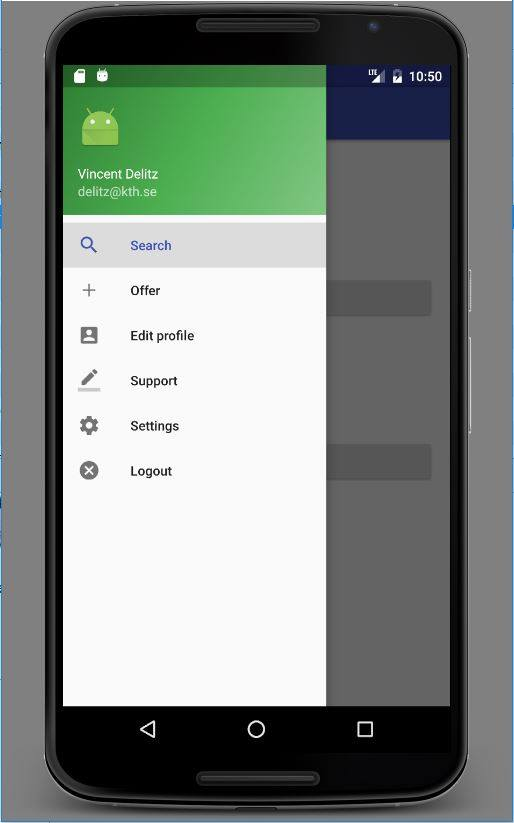
\includegraphics[width=0.4\textwidth]{jpg/android-start-page-1.jpg}
	\caption{Start page}
	\label{figure:start-page}
\end{figure}

\begin{figure}
	\centering
	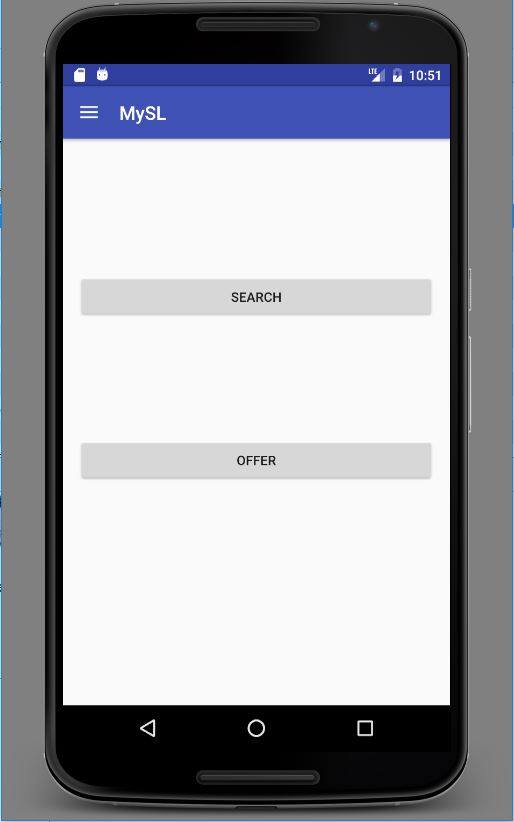
\includegraphics[width=0.4\textwidth]{jpg/android-start-page-2.jpg}
	\caption{Start page}
	\label{figure:start-page}
\end{figure}

\begin{figure}
	\centering
	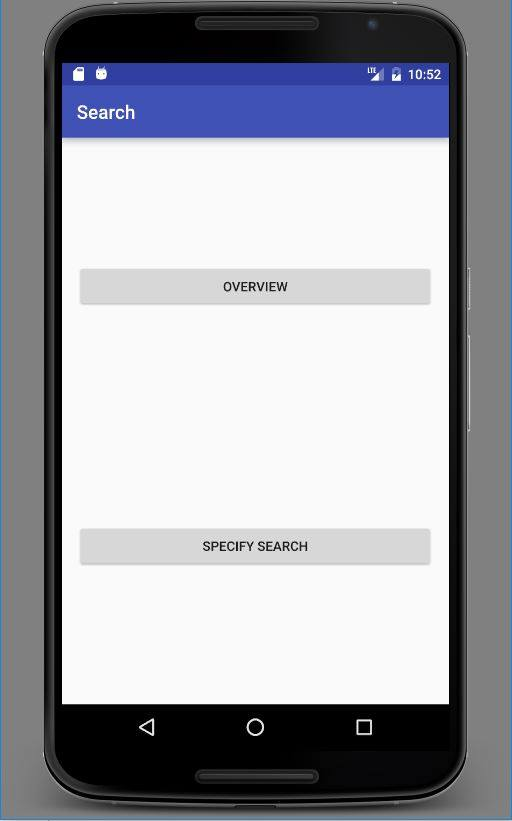
\includegraphics[width=0.4\textwidth]{jpg/android-search-page.jpg}
	\caption{Search page}
	\label{figure:search-page}
\end{figure}

\begin{figure}
	\centering
	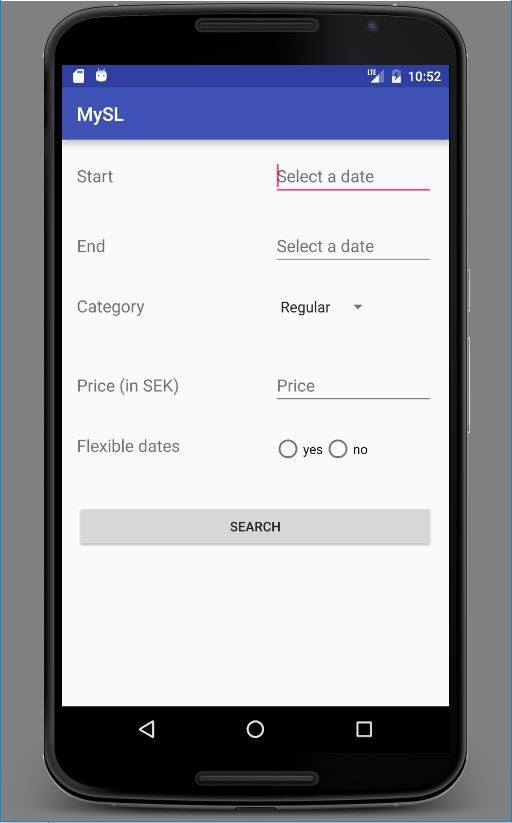
\includegraphics[width=0.4\textwidth]{jpg/android-specify-search-page.jpg}
	\caption{Specify search page}
	\label{figure:specify-search-page}
\end{figure}

\begin{figure}
	\centering
	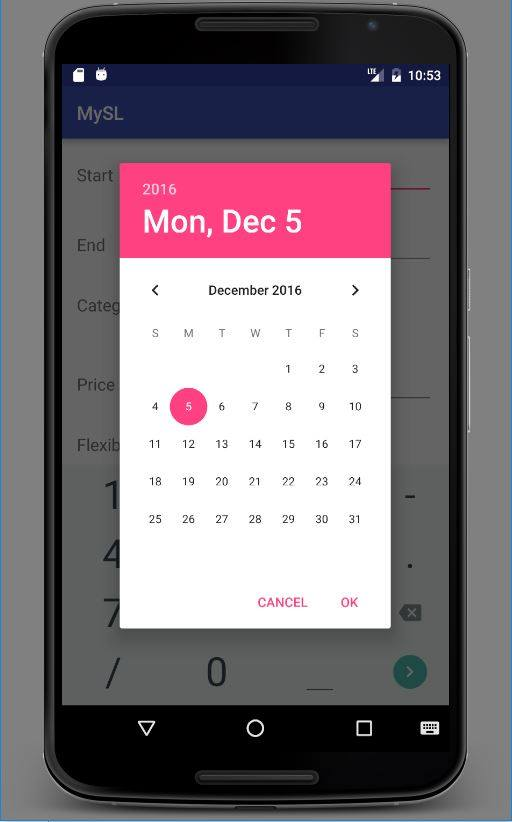
\includegraphics[width=0.4\textwidth]{jpg/android-calendar.jpg}
	\caption{Calendar}
	\label{figure:calendar}
\end{figure}

\begin{figure}
	\centering
	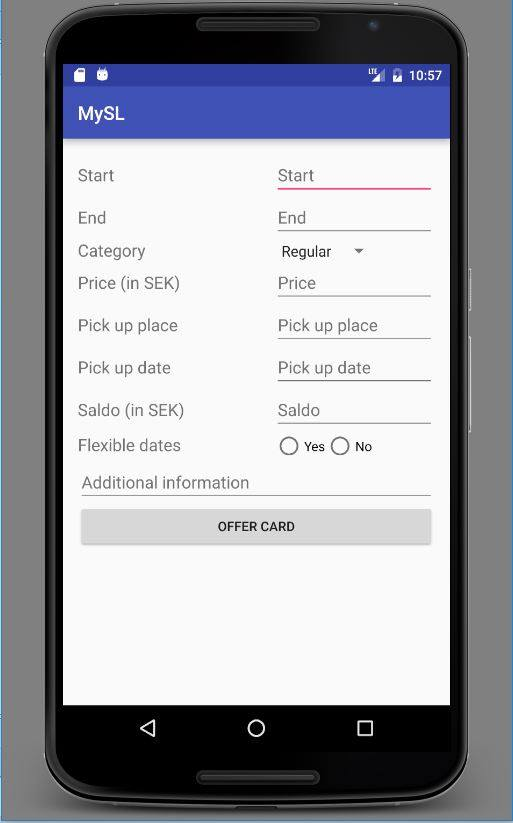
\includegraphics[width=0.4\textwidth]{jpg/android-offer-page.jpg}
	\caption{Offer page}
	\label{figure:offer-page}
\end{figure}

\end{appendices}

\end{document}